\documentclass[12pt,letterpaper,twoside]{article}

\newif\ifsolution\solutiontrue %include solutions
%\newif\ifsolution\solutionfalse % omit solutions
\usepackage{cme211}
\usepackage{multicol}

\begin{document}

Concepts introduced: command line (terminal and shell), remote
computing, textfiles and editors, Python, extensible scripts.

\section{Introduction to Command Line}
A \href{https://en.wikipedia.org/wiki/Command-line_interface}{command line interface (CLI)} 
is a convenient and powerful way to interact with
a computer.  It often takes a bit of adjustment for a person who is used to
\href{https://en.wikipedia.org/wiki/Graphical_user_interface}{graphical user interfaces (GUI)} 
to get up and running with CLIs.  However, the
investment is \emph{always} worth it.  CLIs make repetition and automation quite
simple.  It is much easier to send your colleague a shell command to achieve a
task compared to a sequence of GUI instructions.

\paragraph{Note}
In all documentation for CME211 the dollar sign symbol (\texttt{\$}) will be
used to indicate a shell command.  All shell commands in these notes (and all
CME211 material) are geared for \texttt{bash}, but will likely work in \texttt{tcsh}.  The
pound symbol (\texttt{\#}) is used to indicate shell comments.  Inline, you might see
something like ``try the command \texttt{\$ pwd}''.  Code blocks (like the following)
will also be extensively used for demonstration.  Note that you don't actually
type the \texttt{\$} before the command.

\begin{lstlisting}[language=bash]
# This is a comment, the $ on the next line is followed by a command.
$ pwd
/Users/andreas_santucci/Dropbox/
# the previous line was output from the pwd command
\end{lstlisting}
\vspace{-8pt}
\subsection{Terminal}
A \emph{terminal}, \emph{terminal emulator}, or \emph{console} is a program that displays
text and handles input. These programs emulate the behavior of physical
\href{https://en.wikipedia.org/wiki/Computer_terminal}{computer terminals} (also
known as dumb terminals) in past computing systems. Users of modern computing
systems often have many terminal windows open at once. In the past, users were
limited to the physical terminal they sat behind.
\vspace{-12pt}
\paragraph{Mac}
On macOS, the built-in terminal program is called \texttt{Terminal.app}.  It is located
in \texttt{/Applications/Utilities}.  One convenient way to start the program is to
search for \texttt{terminal} using Spotlight.
\vspace{-12pt}
\paragraph{Windows} On Windows operating systems, the built-in terminal program is called the 
\texttt{Command Prompt}. You may access it by navigating through 
\texttt{Start -> All Programs -> Accessories -> Command Prompt}.
\vspace{-12pt}
\paragraph{Unix} If you're on a Unix operating system already, you likely know how to open 
a terminal. In Ubuntu, for example, you can simply use the keyboard shortcut \texttt{Ctrl - Alt + T}.

\subsection{Shell}
A \emph{shell} is a program that executes commands from the user and displays the
result.  There are many different shell programs out there.  E.g. \href{https://en.wikipedia.org/wiki/Bash_(Unix_shell)}{\texttt{bash}} is quite
popular; it's been around since 1989 and is the default on macOS and most Linux distributions.
For a time, \texttt{tcsh} was the default \emph{shell} on Farmshare systems. It is possible to change
the login shell with the \texttt{chsh} command.

\begin{center}
  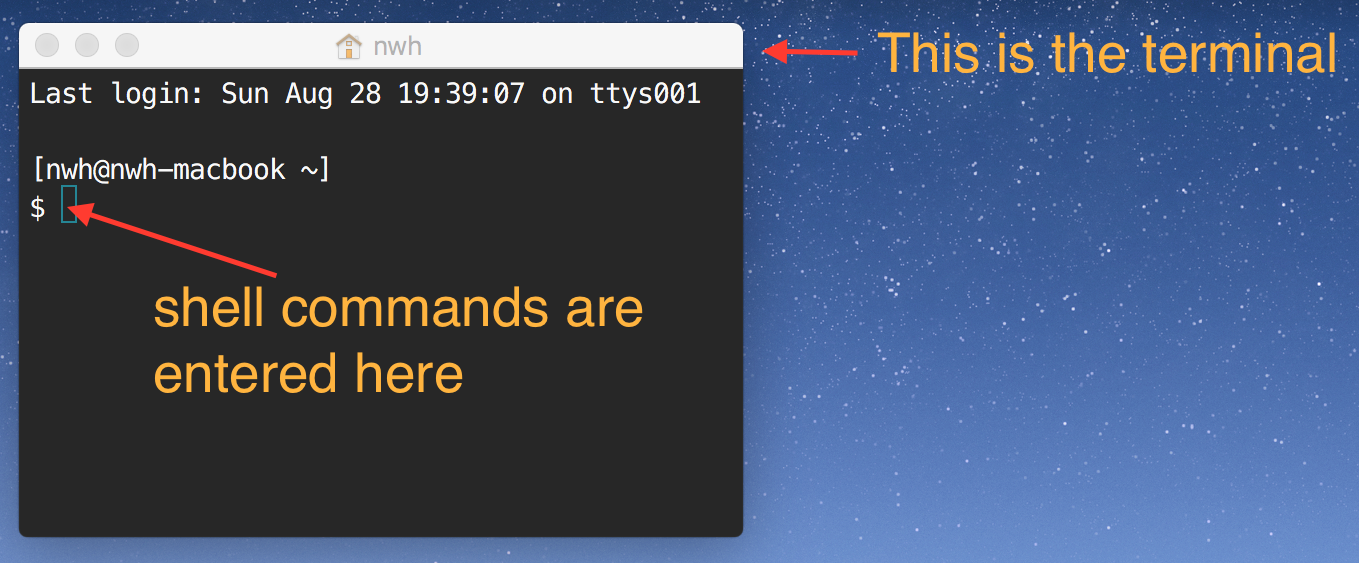
\includegraphics[scale=0.3]{fig/terminal-shell}
\end{center}

\paragraph{Windows}
If you're on Windows 10, I recommend going ahead and 
\href{https://www.microsoft.com/en-us/p/ubuntu/9nblggh4msv6?activetab=pivot:overviewtab}
{installing Ubuntu} on your machine. This will allow you to access all of the Unix 
development tools that we teach.\footnote{While the Command Prompt offered in Windows is still a terminal, it doesn't subscribe to the Unix tool-chain that we teach. Attempts to use something like \texttt{Powershell} will not be amenable to our class as the commands are different and don't directly translate from one tool to another.} If you don't have Windows 10, you can try something like 
\href{https://www.cygwin.com/}{cygwin} or \href{http://www.mingw.org/}{mingw}. The easiest route is to simply use secure shell to access a remote resource, see section \ref{ssh_tools}.
\vspace{-8pt}
\section{Navigating a Command Line Interface}
A \emph{path} specifies the location of a file or directory in a file system
hierarchy.  On unix-like systems (e.g. macOS and Linux) a single slash 
(\texttt{/})
indicates the very top (or root) of the file system.  In longer path names,
directories are separated by slashes.  The last item (lacking a slash) may be
either a file or a directory.  If a path ends with a slash, it's a
directory.
\begin{itemize}
 \item \texttt{/Users/asantucci/Downloads}: this is the downloads directory on my Mac.
 \item \texttt{/Users/asantucci/Downloads/}: this is also the downloads directory on my Mac.  Note
  the trailing slash to indicate that \texttt{Downloads} is a directory.
 \item \texttt{/Users/asantucci/Downloads/syllabus.pdf}: this is the path to a downloaded PDF.
 \item \texttt{\textasciitilde/Downloads}: this is the downloads directory on my Ubuntu machine.
\end{itemize}


Shell commands are executed relative to a \emph{working directory}.  Usually, when
a shell first starts, the working directory is the user's home directory.

\begin{itemize}
\item \texttt{pwd} - print working directory
\item \texttt{cd} - change directory
\end{itemize}

Special directory aliases:

\begin{itemize}
\item \texttt{\~} - user's home directory
\item \texttt{..} - directory one higher in filesystem
\item \texttt{.} - alias for working directory
\end{itemize}

The command \texttt{\$ cd -} changes to the previous directory.

\paragraph{Avoid spaces in directory and file names} 
It is best to not use spaces in directory or file names.  Most shell programs
use a space as a delimiter between commands and arguments.  Thus, spaces in file
or directory names need to be escaped or quoted -- a thing that is easy to
forget.

For example, let's say we have a directory called \texttt{my docs}.  If we try to
enter the directory with \texttt{cd} with out handling the space, we get an error:

\begin{lstlisting}[language=bash]
$ cd my docs
-bash: cd: my: No such file or directory
\end{lstlisting}

To make this work, we can either quote the directory name:

\begin{lstlisting}[language=bash]
$ cd "my docs"
\end{lstlisting}

Or escape the space with a backslash:

\begin{lstlisting}[language=bash]
$ cd my\ docs
\end{lstlisting}

\subsection{Looking at things}
\begin{itemize}
\item \texttt{ls} - list files in directory
\item \texttt{cat} - dump a file to terminal
\item \texttt{less} - open file in a ``pager'' (hit `q' to quit)
\item \texttt{file} - inspect file type
\end{itemize}

\subsection{Manipulating files}
\begin{itemize}
\item \texttt{cp} - copy files and directories
\item \texttt{mv} - move or rename files and directories
\item \texttt{rm} - remove files and directories
  (\textbf{be careful:} files cannot be recovered after \texttt{rm})
\item \texttt{touch} - create file or update timestamp
\item \texttt{mkdir} - create directories
\end{itemize}

\subsection{Inspecting commands}

\begin{itemize}
\item \texttt{type} - Display information about command type
\item \texttt{which} - Locate a command
\item \texttt{help} - Display reference page for shell builtin
\item \texttt{man} - Display an on-line command reference (hit `q` to quit)
\end{itemize}

\subsection{Quitting a command}

Sometimes you need to terminate a command.  This is often possible with the
\texttt{ctrl-c} keyboard command.  In documentation you might see this represented as \texttt{\^} \texttt{C}, where \texttt{\^} is a symbol indicating the `ctrl` key.

\paragraph{Resources}

\begin{multicols}{2}
\small
\begin{itemize}
\item \href{http://linuxcommand.org/}{http://linuxcommand.org/}
\item \href{http://www.pixelbeat.org/cmdline.html}{http://www.pixelbeat.org/cmdline.html}
\item \href{http://software-carpentry.org/}{http://software-carpentry.org/}
  \item \href{http://swcarpentry.github.io/shell-novice/}{http://swcarpentry.github.io/shell-novice/}
  \item \href{https://www.youtube.com/watch?v=hAHJ0xGKMBk}{https://www.youtube.com/watch?v=hAHJ0xGKMBk}
\end{itemize}
\end{multicols}

\section{Remote Computing}
Often various resources (data, programs, high performance computing) are located
somewhere other than the computer we have in front of us.  There are many tools
and methods for accessing remote computing resources.  In CME211, we will use
\href{https://en.wikipedia.org/wiki/Secure_Shell}{\texttt{ssh}} 
to access the shared computing resources managed by 
\href{https://srcc.stanford.edu/}{Stanford Research Computing}.  In particular, we will be using the \texttt{rice} servers on
the \href{https://web.stanford.edu/group/farmshare/cgi-bin/wiki/index.php/Main_Page}
{Farmshare System}.

\paragraph{Structure of Rice}
The \texttt{rice} servers are accessed through the address \texttt{rice.stanford.edu}.  The
``master node'' is called \texttt{rice}`.  This will send users to one of the worker
nodes, designated \texttt{riceXX} where \texttt{XX} is a number.\footnote{We previously used 
a cluster call \texttt{corn}, whence the text within the graphic presented is outdated.}

\begin{center}
  \centering
  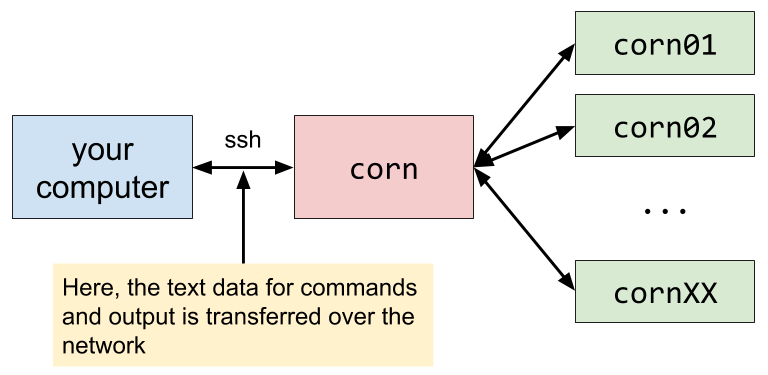
\includegraphics[scale=0.35]{fig/remote-computing}
\end{center}

\paragraph{Logging into a Remote Computer}
\texttt{ssh} stands for ``secure shell''.  The program encrypts the communication between
client and server.  The command to log into `rice` via ssh is:

\begin{lstlisting}[language=bash]
$ ssh [stanford_username]@rice.stanford.edu
\end{lstlisting}

Here, \texttt{stanford\_username} needs to be replaced by your username.  SSH will
then attempt to locate the server, authenticate the user, and provide access
to a shell.

Here is the terminal output when I log into `rice.stanford.edu`.

{
  \footnotesize
\begin{lstlisting}[language=bash]
$ ssh santucci@rice.stanford.edu
Warning: Permanently added the RSA host key for IP address
         `171.67.216.71' to the list of known hosts.

santucci@rice.stanford.edu's password:
Authenticated with partial success.
Duo two-factor login for santucci
Enter a passcode or select one of the following options:

1. Duo Push to XXX-XXX-XXXX
2. Phone call to XXX-XXX-XXXX
3. SMS passcodes to XXX-XXX-XXXX

Passcode or option (1-3): 1
Success. Logging you in...
Welcome to Ubuntu 16.04.5 LTS (GNU/Linux 4.15.0-33-generic x86_64)
# ... many lines omitted ...
For questions or concerns, please contact:
 research-computing-support@stanford.edu

[santucci@rice06 ~] $ pwd
/home/santucci
\end{lstlisting}
}

For more information on SSH, see \texttt{\$ man ssh}, where \texttt{man} is the ``manual'' or ``help'' 
command, useful for fetching documentation for a particular command.

\subsection{Transfering Files (to and from \texttt{rice}) using \texttt{scp}}

The \texttt{scp} (stands for ``secure copy'') tool can be used to copy files to and from
a remote computer running an SSH server.  The following command will copy from
\texttt{source\_file} to \texttt{dest\_file}:

\begin{lstlisting}[language=bash]
$ scp source_file dest_file
\end{lstlisting}

If one (or both) of the files is on a remote computer, then the user and server
address must be specified.  For example, I could copy the file \texttt{demo/doggo.txt}
to my home directory on \texttt{rice} with the following command:

\begin{lstlisting}[language=bash]
$ scp demo/doggo.txt santucci@rice.stanford.edu:~/
# authentication
doggo.txt                                      100%  187     0.2KB/s   00:00
\end{lstlisting}

Note the colon (\texttt{:}) between the server name and path in the above \texttt{scp}
command.

Now looking on \texttt{rice}:

\begin{lstlisting}[language=bash]
[santucci@rice06 ~]
$ ls -1
afs-home
doggo.txt
\end{lstlisting}

\subsection{Farmshare user directory}

The Farmshare remote computing resource offers another location for users to
store files known as the ``Farmshare user directory''.  This is located at
\texttt{/farmshare/user\_data/[sunet\_id]}.  For example, my \texttt{sunet\_id} is \texttt{santucci},
therefore my Farmshare user directory is \newline 
\texttt{/farmshare/user\_data/santucci}.

Some important notes from the \href{https://web.stanford.edu/group/farmshare/cgi-bin/wiki/index.php/User_Guide}{Farmshare User Guide}:

\begin{itemize}
\item  Your Farmshare user directory will likely **not exist** the first time you
login.  A script will run and notice your login and create the directory within
about 30 minutes of your first Farmshare login.

\item  \texttt{/farmshare/user\_data} is \textbf{NOT} backed up.  Make sure your push your work to
GitHub on a regular basis.  You will learn how to do this in HW0.

\item  Space is limited on \texttt{/farmshare}.  There currently is no quota system.  Keep
your Farmshare user directory under \texttt{5GB}.
\end{itemize}

You can \texttt{scp} files directly to your Farmshare user directory.  For example
(from the local \texttt{lecture-00} directory):

{
  \footnotesize
\begin{lstlisting}[language=bash]
$ echo $HOSTNAME
santucci-mbpro.local    # this is my laptop
$ pwd
/Users/santucci/git/cme211-notes/lecture-00
$ scp demo/doggo.jpg santucci@rice.stanford.edu:/farmshare/user_data/santucci/
# authentication
doggo.jpg                                100%  770KB 770.3KB/s   00:00
$ ssh santucci@rice.stanford.edu
# authentication
# now logged into rice.stanford.edu
$ echo $HOSTNAME
rice23.stanford.edu
$ cd /farmshare/user_data/santucci/
$ ls
doggo.jpg
\end{lstlisting}
}


\vspace{-8pt}
\subsection{Other Tools}
\label{ssh_tools}
There are numerous software tools for working with files on remote computing
systems.

There web utilities, \textbf{\emph{accessible from any OS}},
e.g.
\href{https://afs.stanford.edu/}{Stanford WebAFS} provides a web interface to
files on Farmshare, and Google has a beta
\href{https://chrome.google.com/webstore/detail/secure-shell-app/pnhechapfaindjhompbnflcldabbghjo?hl=en}{Chrome-based SSH client}.

Here is a list of \textbf{\emph{Windows specific}} GUI based
tools to for accessing remote computers:

\href{https://uit.stanford.edu/software/securecrt}{SecureCRT},
\href{https://uit.stanford.edu/software/securefx}{SecureFX},
\href{http://www.chiark.greenend.org.uk/~sgtatham/putty/download.html}{PuTTY}, and
\href{https://www.bitvise.com/ssh-client}{Bitvise SSH client}.

The \textbf{\emph{Mac OS}} comes with \texttt{ssh} and \texttt{scp}.  The program Fetch provides a GUI for file
transfer: \href{https://uit.stanford.edu/software/fetch}.  The \texttt{rsync} command may
be used to sync an entire directory:

\begin{lstlisting}[language=bash]
$ rsync -avz -e ssh remoteuser@remotehost:/remote/dir /this/dir/
\end{lstlisting}

Search for \href{https://www.google.com/webhp?q=rsync%20over%20ssh#safe=off&q=rsync+over+ssh}{rsync over ssh} for more information on this.

\vspace{-8pt}
\section{Text Files}
\vspace{-8pt}

A \href{https://en.wikipedia.org/wiki/Text_file}{\emph{text file}}
is simply a sequence of characters that can be opened by any
\href{https://en.wikipedia.org/wiki/Text_editor}{\emph{text editor}}.  
In scientific computing and data science applications, text
files can be used for a variety of tasks:

\begin{multicols}{2}
\begin{itemize}
\item Publication and presentation with \href{https://www.latex-project.org/}{\LaTeX} (\texttt{.tex} file extension)
\item Dataset storage in comma-separated value files (\texttt{.csv})
\item Object serialization with \href{http://www.json.org/}{JSON} (\texttt{.json})
\item Websites (\texttt{.html}) or \href{http://daringfireball.net/projects/markdown/}{markdown files} (\texttt{md}).
\item Graphics with tools like \href{https://developer.mozilla.org/en-US/docs/Web/SVG}{SVG} or 
\href{http://www.texample.net/tikz/}{TikZ}.
\item Source code in any language, CME211 will use Python (\texttt{.py}) and C++ (\texttt{.cpp})
\item Tools for \href{http://www.implicitcad.org/}{3d models}.
\item Software build systems with \href{https://www.gnu.org/software/make/}{GNU Make} or \href{https://cmake.org/}{CMake}.
\item \href{http://lilypond.org/text-input.html}{Music notation}
\end{itemize}
\end{multicols}

One benefit of working with text files is that they can be checked into
version control systems and easily compared to previous versions.  It is also
possible to check \href{https://en.wikipedia.org/wiki/Binary_file}{binary files} 
into a version control system, but it is not as
easy to find the differences from previous versions;
some examples of binary files include
\texttt{.zip}, \texttt{.jpg}, \texttt{.xls}, \texttt{.docx}.

\vspace{-14pt}
\subsection{Text Editors}

Text editors that work in a terminal include (my personal favorite)
\href{https://www.gnu.org/software/emacs/}{Emacs},
\href{http://www.vim.org/}{Vim}, and
\href{https://www.nano-editor.org/}{Nano}. 

GUI Based text editors include \href{https://atom.io/}{Atom}, 
\href{https://www.sublimetext.com/}{Sublime Text},
\href{https://code.visualstudio.com/}{Visual Studio Code},
and
\href{http://www.barebones.com/products/textwrangler/}{TextWrangler}.\footnote{
  \textbf{Caution:} 
  you likely will feel more comfortable using a GUI based text editor
  \emph{at first}. However, I strongly recommend learning to at least
  feel comfortable working out of a terminal editor: they are guaranteed
  to be available on any Unix system, and they have existed for decades;
  the ``features''  that come with paid versions of GUI counterparts
  often include functionality that is often decades old and freely
  available if you're comfortable learning to read documentation.
If you want something more
modern, consider
\href{https://github.com/xi-editor/xi-editor}{xi}.
}
\vspace{-28pt}
\section{Interacting with Python}
\vspace{-8pt}
\begin{itemize}
\item Python is a
  \href{https://en.wikipedia.org/wiki/High-level_programming_language#Features}{high
    level language} that typically runs in an
  \emph{interpreter}.\footnote{You may have heard the expression
    \href{https://en.wikipedia.org/wiki/Low-level_programming_language\#Assembly}{low
      level language}, which allow the programmer to interface with
    the computer's instruction set architecture; this means dealing
    with registers, memory addresses, and call stacks. A high level
    language, in contrast, allows the programmer to think instead
    about variables, arrays, subroutines. Higher level languages focus
    on usability over efficiency.}
\item
  An \emph{interpreter} is a program that
  executes statements from a high level language.
\item
  Examples of high level interpreted languages: Python, R, Matlab, Perl,
  JavaScript
\item
  The most widely used 
  \href{https://docs.python.org/3/reference/introduction.html#alternate-implementations}
  {Python interpreter (or implementation)} 
  is called \textbf{CPython}. It
  is written in C. There are others, for example \textbf{Jython} and
  \textbf{IronPython}. It is fairly easy (with experience) to access
  code written in C from \textbf{CPython}. 

  There's even
  \href{https://pypy.org/}{Pypy},  an implementation of Python written
  in Python.
\item
  Python now has a 
  \href{https://en.wikipedia.org/wiki/Python_(programming_language)#History}{long
    history}.
  It started in '89 as a project to keep Guido van Rossum occupied
  during the week around Christmas; version 1.0 was released in 1994.
\item
  This class will use Python 3, which has 
  \href{https://sebastianraschka.com/Articles/2014_python_2_3_key_diff.html#sections}
  {important differences from Python2}.
\end{itemize}

\vspace{-8pt}
\subsection{Getting started}
\vspace{-8pt}

Let's log into \texttt{rice.stanford.edu}, start the
Python 3 interpreter, and execute Python code.

\begin{enumerate}
\item Use SSH to login with \texttt{ssh [sunet\_id]@rice.stanford.edu}
\item Run the Python 3 interpreter with \texttt{\$\ python3}
\item Execute the python statement
  \texttt{>>> print("Hello World!")}.
\end{enumerate}

\subsubsection{Interpreter}

\begin{itemize}
\item An \emph{interpreter} is a program that reads and executes commands.
\item It is also sometimes called a REPL or read-evaluate-print-loop.
\item One way to interact with Python is to use the interpreter.
\item This is useful for interactive work, learning, and simple testing.
\item When you see a \texttt{\$} in code blocks, it typically indicates a
  shell command. For example: 

\begin{verbatim}
$ ls -1 *.md
0-outline.md
1-values-variables-types.md
2-strings.md
3-numbers.md
\end{verbatim}

\item
  A \texttt{>>>} in
  code blocks signifies a command for the Python
  interpreter.
\item
  The basic Python interpreter is good for simple computations or
  checks. \href{https://ipython.org/}{IPython} provides more
  functionality (e.g. tab completion, syntax highlighting); see \texttt{\$\ ipython3}.
\end{itemize}

\subsubsection{Python as a calculator}

In the Python 3 interpreter:

\begin{multicols}{2}
\small
\begin{verbatim}
>>> 4+7
11
>>> 55*2
110
>>> 9-1.4
7.6
# Next, we show differences between 
# (floor) division
>>> 5/3
1.6666666666666667
>>> 5//3
1
>>> -5//3
-2
>>> 5.0/3
1.6666666666666667
>>> 5.0//3
1.0
>>> 5 % 3
2
\end{verbatim}
\end{multicols}

Surprised?
\begin{itemize}
\item
  Division between two integers with \texttt{/} returns a floating point
  number.
\item
  The operator \texttt{//} performs floor division (rounds down).
\item
  The \texttt{\%} (modulus) operator
  returns the remainder for integer division.
\end{itemize}

\hypertarget{integers-and-floating-point}{%
\subsubsection{Integers and floating
point}\label{integers-and-floating-point}}

We'll discuss details of computer
representation of numeric values later, but for now:

\begin{itemize}
\item
  It is best to think of integers as being represented exactly over a
  fixed range.\footnote{This is not really true in current versions of Python,
  but will be true in C++.}
\item
  Floating point numbers are \emph{approximations} of real numbers over
  a limited range.
\item
  Floating point number range is not continuous: the size of gaps between
  adjacent floating point numbers depend on the scale.\footnote{The gap between
  \texttt{1.0} and the next representable floating point number is
  smaller than the gap between \texttt{1.0e50} and the next
  representable floating point number.}
\item
  These things matter; bad numerical computing has resulted in \href{https://www.ima.umn.edu/~arnold/disasters/}{disasters}.
\end{itemize}
\vspace{-18pt}
\subsubsection{Exiting the interpreter}
We simply use either \texttt{ctrl-d} or \texttt{exit()}
{
\footnotesize
\begin{verbatim}
$ python3
Python 3.5.2 (default, Jun 29 2016, 13:43:58)
[GCC 4.2.1 Compatible Apple LLVM 7.3.0 (clang-703.0.31)] on darwin
Type "help", "copyright", "credits" or "license" for more information.
>>> exit
Use exit() or Ctrl-D (i.e. EOF) to exit
>>> exit()
\end{verbatim}
}
\vspace{-8pt}
\subsubsection{Python scripts}

\begin{itemize}
\item
  A more convenient way to interact with Python is to write a script
\item
  A Python script is a text file containing Python code
\item
  Python script file names typically end in \texttt{.py}
\end{itemize}
\vspace{-8pt}
\textbf{Let's create our first script:}
\vspace{-8pt}
\begin{itemize}
\item
  Log into \texttt{rice.stanford.edu}
\item
  Create a text file named \texttt{firstscript.py} with your favorite
  text editor. 

  (\texttt{\$\ nano\ firstscript.py} is a good choice)
\item
  Insert the following Python code into \texttt{firstscript.py}:
  {\small
  \begin{python}
    print("Hello from Python")
    print("I am your first script!")
  \end{python}
  }
\item
  Execute the command \texttt{\$\ python3\ firstscript.py}
\end{itemize}

Note the use of the \texttt{\$\ python3} command. On many systems the
command \texttt{\$\ python} will start the Python 2 interpreter. For
this simple example, the behavior will be the same. In general, this is
not the case Python versions 2 and 3 have
\href{https://docs.python.org/3/whatsnew/3.0.html}{many differences}.

\subsection{Scripts are Extensible}
Let's write a simple Python script to compute the first \texttt{n}
numbers in the Fibonacci series. As a reminder, each number in the
Fibonacci series is the sum of the two previous numbers. Let
$F(i)$ be the $i$th number in the series. We define
$F(0) = 0$ and $F(1) = 1$, and
$F(i) = F(i-1) + F(i-2)$ for all $i \geq 2$.
Numbers \texttt{F(0)} to \texttt{F(n)} can be computed with the
following Python code:

\begin{python}
n = 10

if n >= 0:
    fn2 = 0
    print(fn2,end=',')
if n >= 1:
    fn1 = 1
    print(fn1,end=',')
for i in range(2,n+1):
    fn = fn1 + fn2
    print(fn,end=',')
    fn2 = fn1
    fn1 = fn
print()
\end{python}

Note, the above code is a preview of Python syntax that we will review
in this course. Now, paste this code into a file named \texttt{fib.py}.

Execute the file with the command \newline 
\texttt{\$\ python3\ fib.py}. The result should like:

\begin{lstlisting}[language=bash]
$ python3 fib.py
0,1,1,2,3,5,8,13,21,34,55,
\end{lstlisting}

To see the utility of scripts, we need to add a bit more code. Change
the first line of \texttt{fib.py} to be:

\begin{python}
import sys
n = int(sys.argv[1])
\end{python}

This will instruct the script to obtain the value of \texttt{n} from the
command line:

\begin{lstlisting}[language=bash]
$ python3 fib.py 0
0,

$ python3 fib.py 5
0,1,1,2,3,5,

$ python3 fib.py 21
0,1,1,2,3,5,8,13,21,34,55,89,144,233,377,610,987,1597,2584,4181,6765,10946,
\end{lstlisting}

We have increased the utility of our program by making it simple to run
from the command line with different input arguments. CME211 homeworks
will work like this.

\subsubsection{Python modules}
If you are familiar with MATLAB or R, you may come to Python and be confused
by:

\begin{python}
sqrt(3)  # --> Yields a NameError: name 'sqrt' not defined.
\end{python}

The Python language does not have a built in \texttt{sqrt} function;
this subroutine exists in the \texttt{math} module.

\begin{python}
import math
math.sqrt(9)
\end{python}

About Python modules:

\begin{itemize}
\item
  A module is a collection of Python resources (functions, variables,
  objects, classes) that can be easily loaded into Python via
  \texttt{import} statements.
\item
  Modules allow for easy code reuse and organization.
\item
  Modules allow the programmer to keep various functionality in
  different namespaces.
\item
  There are a large number of modules in the Python Standard Library:
  \url{https://docs.python.org/3/library/index.html}
\item
  It is often useful to explore the Python documentation in the
  interpreter. See \newline
  \texttt{>>> help(math)} and
  \texttt{>>> help(math.sqrt)}
  from the interpreter.
\end{itemize}

\subsubsection{Printing}

The Python interpreter (and Jupyter Notebook) 
will echo the output of the last (non-assignment)
statement in a code block:

\begin{python}
1+1  # Echos --> 2.
5+5  # Echos --> 10.
\end{python}

\begin{python}
myvar = 101  # Nothing is printed to console.
\end{python}

You can use the \texttt{print()} function if you wish to inspect its contents.
\begin{python}
a = 99
print(a)    # Echos --> 99.
\end{python}

By default, \texttt{print()} adds a new line character at the end for
printing.

\begin{python}
print("hi")           # These contents are ...
print("cme211")       # ... printed on two lines.
\end{python}

This behavior can be changed by setting the \texttt{end} keyword
parameter in the print function.

\begin{python}
print("hi", end = ' ')  # Now prints a space after "hi" instead of a newline ('\n').
print("cme211")         # The result looks like -- "hi cme211" on its own line.
\end{python}

The \texttt{print()} function can print several strings at once on the
same line:

\begin{python}
print("apple", "bananna", "orange")
\end{python}

The default separator is a space. This can be changed by setting the
\texttt{sep} keyword parameter:

\begin{python}
print("apple", "bananna", "orange", sep = ", ")  # Add a comma in addition to a space.
\end{python}

Python strings can be ``formatted'' with the \texttt{format} method:

\begin{python}
r = 10
print("The area of a circle of radius {} is {}".format(r, math.pi * math.pow(r, 2)))
\end{python}

The curly braces (\texttt{\{\}}) get replaced by the arguments to
\texttt{format()} in order.

\subsection{Values, types, and variables}

\subsubsection{Values}
A value is the fundamental thing that a program manipulates or uses to
perform operations. A value is data.

Here is a string value.

\begin{python}
"Hello, world!"
\end{python}

Here are some numeric values.

\begin{python}
42
12.34
\end{python}

Here the \emph{only two} Boolean values.
\begin{python}
True
False
\end{python}

Values have types associated with them.

\subsubsection{Types}

In Python there are several fundamental data types:

\begin{itemize}
\item
  \texttt{bool}: with values \texttt{True} and \texttt{False}
\item
  \texttt{str}: for strings like \texttt{"Hello\ world"}
\item
  \texttt{int}: for integers like \texttt{1}, \texttt{42}, and
  \texttt{-5}
\item
  \texttt{float}: for floating point numbers like \texttt{96.8}
\end{itemize}

Python has a \texttt{type()} function to determine the type of a value.

\begin{python}
  type(55)               # <class 'int'>
  type(-101.5)           # <class 'float'>
  type(False)            # <class 'bool'>
  type("Hi there")       # <class 'str'>
\end{python}

In many programming languages, the terms \texttt{class} and \texttt{type}
are either synonymous or at least closely related.

\subsubsection{Variables}

One of the most basic and powerful concepts in programming is that of
  a variable, which associates a name to a value.

\begin{python}
message = "hello world!"
n = 42
e = 2.71
print(n)  # Echos 42.
\end{python}

The last expression shows its possible to print a variable. Everything
after the \# symbol is part of a comment that is disregarded by the interpreter.

It is almost always preferred to use variables over values. Why?
Easier to update code
Easier to understand code (useful naming)
For example, What does the following code do:

\begin{python}
4.2 * 3.5
\end{python}

Yeah, we're multiplying two scalar values, but what's the purpose of
the computation?
If the values are assigned to variables with meaningful names, we
might have something like the following.

\begin{python}
length = 4.2
height = 3.5
area = length * height
print(area)
\end{python}

Now a person reading the code has a good idea of what the values
represent and what the output of the code means.

\subsubsection{Variable naming}

The name associated with a variable is referred to as an
\emph{identifier}
Variables names must start with a letter or an underscore, such as

\begin{python}
_underscore
underscore
\end{python}

The remainder of your variable name may consist of letters, numbers
and underscores


\begin{python}
password1 = "..."
n00b = math.pi
under_scores = "__"
\end{python}

Names are case sensitive, i.e. \texttt{case\_sensitive},
\texttt{CASE\_SENSITIVE}, and \texttt{Case\_Sensitive} are all different.

\subsubsection{Variable naming style}

One letter characters such as \texttt{a}, \texttt{b}, and \texttt{c}
are too short and not at all descriptive (in general) for meaningful
variable names; I've had coworkers do this and it's difficult for them
to debug their own logic errors. 

On the other hand, something like
\texttt{number\_of\_particles\_in\_target\_region} is too long; I've
also had coworkers do this and it leads to simple expressions looking
needlessly complex. 

A better balance might be
\texttt{num\_target\_particles}. Perhaps instead of underscore, we
prefer camel case i.e. \texttt{numTargetParticles}.
This is quite important for code readability. People think about this a
lot. See:
\href{https://www.python.org/dev/peps/pep-0008/\#naming-conventions}
{naming conventions in Python}.

\subsubsection{Important: don't override built-in names}

\begin{python}
print(abs(-7))
abs = "Must code"
print(abs(-4))      # TypeError: 'str' object is not callable.
\end{python}

\subsubsection{Exercise: mortgage calculator}

Let's write a simple mortgage calculator to compute the monthly payment
for a mortgage.

Here are the parameters:

\begin{itemize}
\item $L$: initial principal or value of the loan
\item $r$: yearly interest rate
\item $c = r/12$: monthly interest rate
\item $n$: term of the mortgage in terms of number of months (30 years
  360 months)
\end{itemize}

The formula to compute the fixed monthly payment is:

\[
P = L \frac{c(1+c)^n}{(1+c)^n-1}
\]

Let's code this in Python:

\begin{python}
# mortgage amount in dollars
L = 100000
# yearly interest rate of 4%
r = .04
c = r / 12
# duration of mortgage in months
n = 360
P = L * (c*(1+c)**n) / ((1+c)**n-1)
print("P = " + str(P))
\end{python}

Note that in Python the notation \texttt{x**y} is used to compute
``\texttt{x} raised to the power \texttt{y}''.

\subsubsection{Exercise for you: reverse mortgage calculator}

Now, write python code to compute the value of the loan given the
monthly payment. The formula is:

\[
L = P \frac{(1+c)^n-1}{c(1+c)^n}
\]

\section{Reading}
From \textbf{The Linux Command Line} by William Shotts: *
\url{http://linuxcommand.org/lc3_learning_the_shell.php\#contents} *
Read section 1, 2, 3, 5, and 6 * Skip sections 4, 7 and above unless
interested

\section{Appendix: Jupyter Notebooks (Not Part of CME211)}
Jupyter Notebooks are great for teaching and interactive work. From the
\href{http://jupyter.org/}{jupyter.org} website:

\begin{quote}
The Jupyter Notebook is a web application that allows you to create and
share documents that contain live code, equations, visualizations and
explanatory text. Uses include: data cleaning and transformation,
numerical simulation, statistical modeling, machine learning and much
more.
\end{quote}

\subsection{Jupyter notebook}
In Jupyter Notebook, code is typed into code blocks:

\begin{python}
print("hello from a code block!")
\end{python}

Code blocks can be re-executed with ease!

You can test Jupyter Notebook in your browser via
\url{https://try.jupyter.org/}. Note that any work you do here will not
be saved.

If you want to install Jupyter Notebook on your computer, I recommend
\href{https://www.continuum.io/downloads}{Anaconda Python} or using 
\href{https://brew.sh/}{brew} if you're on a Mac OS. Make sure to
install the correct version corresponding to Python 3.x.

\begin{itemize}
\item
  We do not formally support Jupyter Notebook in this class. We show it to the class
  because it is a very useful tool. If you want to look into it,
  there's some great tutorials online.
\item
  The teaching staff is not responsible for helping you set up Jupyter
  Notebook on your computer. Python 3 on \texttt{rice.stanford.edu} is
  the supported computing environment!
\item
  All Python work for CME211 must be submitted as Python scripts
  (\texttt{.py} files) that can be executed via the command line. We
  will not accept notebook format (\texttt{.ipynb}).
\end{itemize}

\paragraph{Jupyter Notebook can render math}

Here is a simple indefinite integral:

\[
\int x\ dx = \frac{1}{2} x^2 + C
\]

Here is an inline equation \(e^{ix} = \cos x + i \sin x\) for any real
number \(x\).

\subsection{Looking ahead with Jupyter Notebooks}

Jupyter notebook is a very useful tool for scientific computing. If you
have a background with Matlab, the following may help you get started
working with Python and NumPy.

Start by importing modules:

\begin{python}
# for 2d plotting
import matplotlib.pyplot as plt
# for numerical computing
import numpy as np
\end{python}

Configure plotting for notebook:

\begin{python}
# tell matplotlib to use the notebook for figures
%matplotlib inline
# tell matplotlib to use svg (they look better than png)
#%config InlineBackend.figure_format = 'svg'
\end{python}

Note: in Jupyter notebook, statements that start with \texttt{\%} are
known as
\href{http://ipython.readthedocs.io/en/stable/interactive/magics.html}{magic
commands}.

A simple plot of 100 random sampled data points:

\begin{python}
plt.plot(np.random.rand(100))
\end{python}

Have a look at the
\href{http://mathesaurus.sourceforge.net/matlab-numpy.html}{``NumPy for
MATLAB Users''} reference. Note that you will have to prefix NumPy
function calls from the reference with \texttt{np.} based on the import
statements above.

It may also be a good idea to skim the following to see what you can
do (not required, simply a foreshadowing)
  \href{http://docs.scipy.org/doc/numpy/reference/}{NumPy reference}, and
  \href{http://docs.scipy.org/doc/scipy/reference/}{SciPy reference}.
 \end{document}
